\section{Observed Flaws}\label{flaws}

% Moved earlier to display nicely in paper
% \flawMnfstsTable{}
% \flawDmnsTable{}

After gathering all these data\footnote{Available in \texttt{ApproachGlossary.csv},
    \texttt{QualityGlossary.csv}, and \texttt{SuppGlossary.csv} at \ifblind{
        [Repository link suppressed]}{
        \url{https://github.com/samm82/TestingTesting}}.}, we find many
flaws. \Cref{fig:flawBars} shows the source tiers (see \Cref{source-tiers})
responsible for these flaws, which reveals a lot about software testing literature:
\begin{enumerate}
    \item Established standards (\Cref{stds}) aren't actually standardized, since:
          \begin{enumerate}
              \item other documents disagree with them \emph{very} frequently and
              \item they are the most internally inconsistent source tier!
          \end{enumerate}
    \item Less standardized (or ``credible''; see \Cref{cred}) documents,
          such as terminology collections and textbooks (\Cref{metas,texts},
          respectively) are also not followed to the extent they should be.
    \item Documents across the board have flaws within the same document,
          between documents with the same author(s), or even with reality%
          \qtodo{Is this too strong of a synonym for ``ground truth''?}!
\end{enumerate}

To better understand and analyze these flaws, we group them by their
manifestations and their domains as defined in \Cref{flaw-def}.
We present the total number of flaws by manifestation and by domain
in \Cref{tab:flawMnfsts,tab:flawDmns}, respectively, where a given
row corresponds to the number of flaws either within that source tier and/or
with a ``more credible'' one (i.e., a previous row in the table; see
\Cref{cred,source-tiers}). We also group these flaws by their explicitness
(defined in \Cref{explicitness}) by counting (Obj)ective and (Sub)jective flaws
separately, since additional context may rectify them.
Since we give each flaw a manifestation \emph{and} a domain, the totals per
source and grand totals in these tables are equal. From these tables, we can
draw some conclusions about \emph{how} the literature is flawed:
\begin{enumerate}
    \item Contradictions are by \emph{far} the most common way for a flaw to
          manifest, which makes sense: if two (groups of) authors do not
          communicate or work with different resources, there is a higher
          chance that they will disagree.
    \item Approach categorizations are the most subjective and one of the most
          common flaw domains, likely due to the lack of standardization
          about what categories to use\ifnotpaper\ (see \Cref{alt-cats}
              for more detailed discussion)\fi.
\end{enumerate}

\ifnotpaper
    \begin{figure}[bt!]
\centering
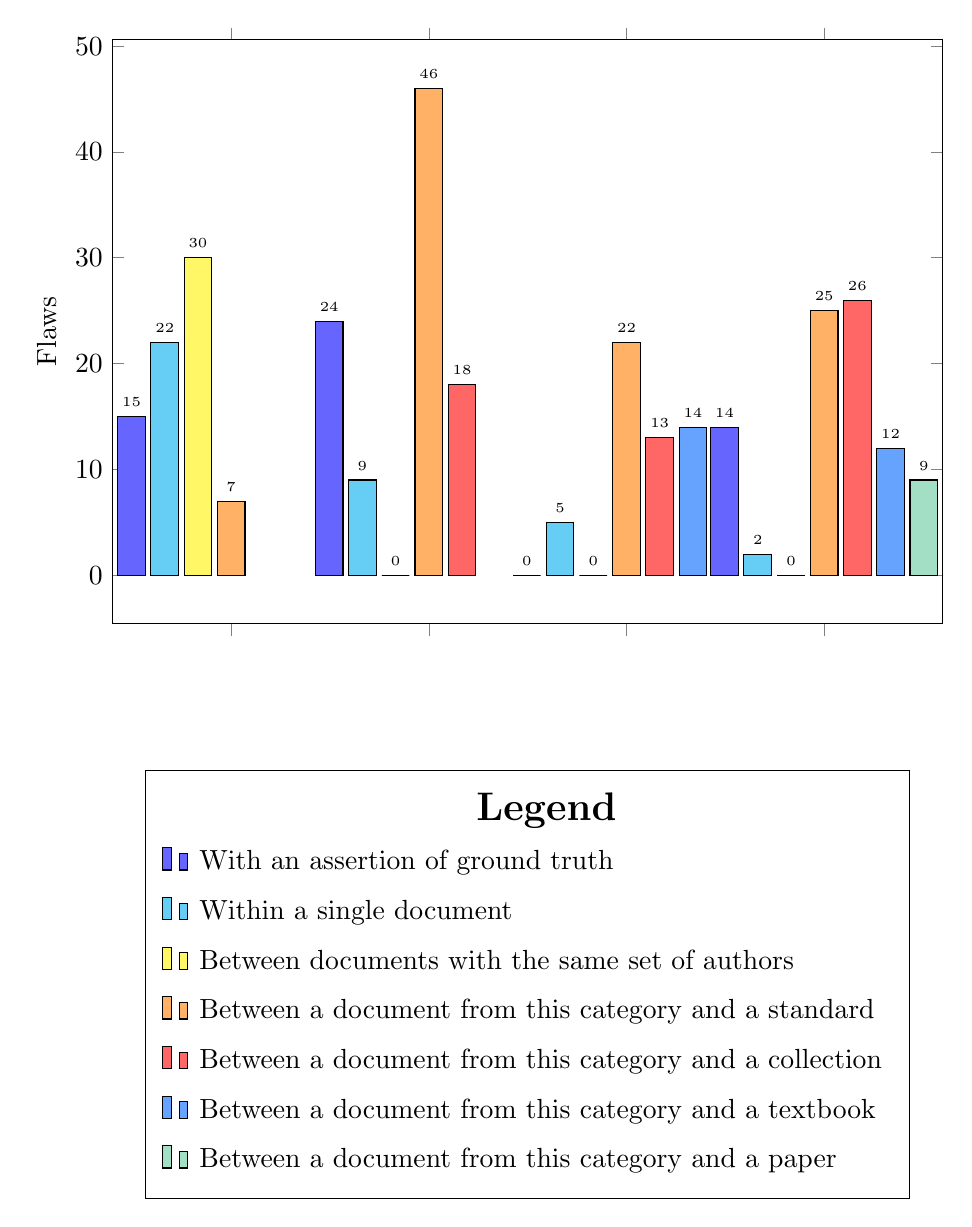
\begin{tikzpicture}
\begin{axis}[
width=\textwidth, height=9cm,
symbolic x coords={std,meta,text,paper},
xtick=data,
xticklabels={{\parbox{0.16\textwidth}{\centering \stds{}}},{\parbox{0.16\textwidth}{\centering \metas{}}},{\parbox{0.16\textwidth}{\centering \texts{}}},{\parbox{0.16\textwidth}{\centering \papers{}}}},
ylabel=Flaws, ybar,
enlargelimits=0.2, enlarge y limits=0.1,
legend style={at={(0.5,-0.25)}, anchor=north, legend columns=1,
inner xsep=6pt,inner ysep=4pt,
nodes={inner sep=4pt,text depth=0.3em},},
legend cell align=left,
nodes near coords,
every node near coord/.append style={font=\tiny},
]
\addlegendimage{empty legend}
\addplot[fill=blue!60] coordinates {(std, 15) (meta, 24) (text, 0) (paper, 14)};
\addplot[fill=cyan!60] coordinates {(std, 22) (meta, 9) (text, 5) (paper, 2)};
\addplot[fill=yellow!60] coordinates {(std, 30) (meta, 0) (text, 0) (paper, 0)};
\addplot[fill=orange!60] coordinates {(std, 7) (meta, 46) (text, 22) (paper, 25)};
\addplot[fill=red!60] coordinates {(meta, 18) (text, 13) (paper, 26)};
\addplot[fill=blue!60!cyan!60] coordinates {(text, 14) (paper, 12)};
\addplot[fill=cyan!60!yellow!60] coordinates {(paper, 9)};
\legend{\hspace{3.4cm} \Large \textbf{Legend},With an assertion of ground truth,Within a single document,Between documents with the same set of authors,Between a document from this category and a standard,Between a document from this category and a collection,Between a document from this category and a textbook,Between a document from this category and a paper}
\end{axis}
\end{tikzpicture}
\caption{Identified flaws by the source tier responsible. Some bars are omitted as they correspond to comparisons we do not make; see \Cref{flaw-cred-compare}.}
\label{fig:flawBars}
\end{figure}

    % \begin{figure*}
\centering
\begin{subfigure}[t]{0.475\textwidth}
\begin{tikzpicture}[thick, scale=0.7, every label/.style={align=left, scale=0.7}]
   \pie[text=legend, sum=auto, hide number, color={blue!60, cyan!60, yellow!60, orange!60}]{
      11/15.7\%,
      29/41.4\%,
      25/35.7\%,
      5/7.1\%
}
\end{tikzpicture}
\caption{Flaws found in \stds{}.}
\label{fig:stdFlawSources}
\end{subfigure}
\hfill
\begin{subfigure}[t]{0.475\textwidth}
\begin{tikzpicture}[thick, scale=0.7, every label/.style={align=left, scale=0.7}]
   \pie[text=legend, sum=auto, hide number, color={blue!60, cyan!60, orange!60, red!60}]{
      19/21.1\%,
      10/11.1\%,
      44/48.9\%,
      17/18.9\%
}
\end{tikzpicture}
\caption{Flaws found in \metas{}.}
\label{fig:metaFlawSources}
\end{subfigure}
\vskip\baselineskip
\begin{subfigure}[t]{0.475\textwidth}
\begin{tikzpicture}[thick, scale=0.7, every label/.style={align=left, scale=0.7}]
   \pie[text=legend, sum=auto, hide number, color={cyan!60, orange!60, red!60, blue!60!cyan!60}]{
      4/6.9\%,
      26/44.8\%,
      14/24.1\%,
      14/24.1\%
}
\end{tikzpicture}
\caption{Flaws found in \texts{}.}
\label{fig:textFlawSources}
\end{subfigure}
\hfill
\begin{subfigure}[t]{0.475\textwidth}
\begin{tikzpicture}[thick, scale=0.7, every label/.style={align=left, scale=0.7}]
   \pie[text=legend, sum=auto, hide number, color={blue!60, cyan!60, orange!60, red!60, blue!60!cyan!60, cyan!60!yellow!60}]{
      10/13\%,
      3/3.9\%,
      23/29.9\%,
      24/31.2\%,
      10/13\%,
      7/9.1\%
}
\end{tikzpicture}
\caption{Flaws found in \papers{}.}
\label{fig:paperFlawSources}
\end{subfigure}
\vskip\baselineskip
\begin{center}
\begin{subfigure}[t]{\linewidth}
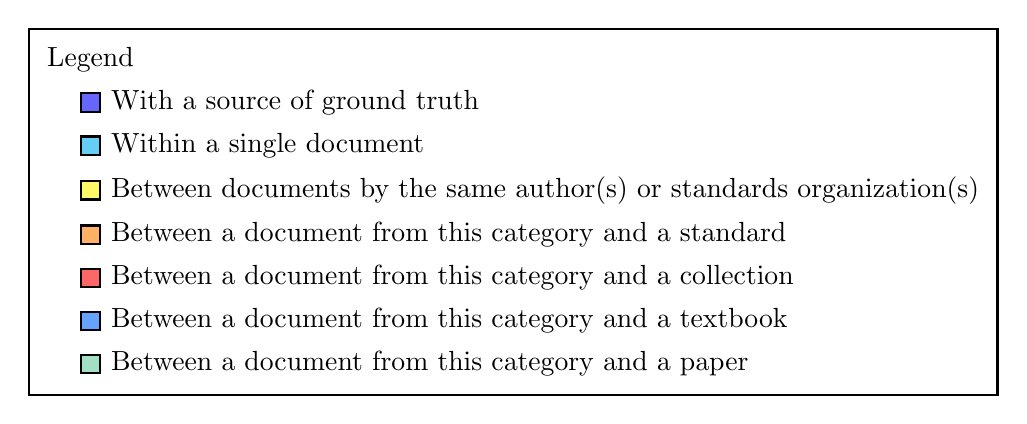
\begin{tikzpicture}
\matrix [thick, draw=black] {
\node[label=center:Legend] {{}}; \\
\node[thick, shape=rectangle, draw=black, fill=blue!60, label=right:{With a source of ground truth}](0) {}; \\
\node[thick, shape=rectangle, draw=black, fill=cyan!60, label=right:{Within a single document}](1) {}; \\
\node[thick, shape=rectangle, draw=black, fill=yellow!60, label=right:{Between documents by the same author(s) or standards organization(s)}](2) {}; \\
\node[thick, shape=rectangle, draw=black, fill=orange!60, label=right:{Between a document from this category and a standard}](3) {}; \\
\node[thick, shape=rectangle, draw=black, fill=red!60, label=right:{Between a document from this category and a collection}](4) {}; \\
\node[thick, shape=rectangle, draw=black, fill=blue!60!cyan!60, label=right:{Between a document from this category and a textbook}](5) {}; \\
\node[thick, shape=rectangle, draw=black, fill=cyan!60!yellow!60, label=right:{Between a document from this category and a paper}](6) {}; \\
};
\end{tikzpicture}
\end{subfigure}
\end{center}
\hfill
\caption{Sources of flaws based on \hyperref[sources]{source tier}.}
\label{fig:flawSources}
\end{figure*}


    % \input{build/flawTable}
    \begin{landscape}
        \flawMnfstsTable{}
        \flawDmnsTable{}
    \end{landscape}

\fi

We summarize the flaws that we discover manually \ifnotpaper (see
    \Cref{aug-flaw-analysis}) \fi in \Cref{flawMnfsts} based on their
manifestation (defined in \Cref{mnfst-def}). This lets us keep flaws that we
automatically uncover \ifnotpaper (see \Cref{auto-flaw-analysis}) \fi separate;
we summarize these based on their domain (defined in \Cref{dmn-def}) in
\Cref{flawDmns}.
\ifnotpaper We list \emph{all} these flaws in \Cref{flaws-full} to balance
    completeness and brevity and denote implicit relations with the phrase
    ``implied by'' in \Cref{tab:parSyns,tab:multiCats,tab:infMultiCats} as
    described in \Cref{explicitness}. \fi Moreover, certain ``subsets'' of
testing contain many interconnected flaws, which we present in subsections as a
``third view'' to keep related information together. Therefore, the counts of
flaws given in \Cref{tab:flawMnfsts,tab:flawDmns} can be thought of as the sum
the flaws we describe by manifestation, domain, and ``subset''. These subsets
include \ifnotpaper operational (acceptance) testing (\Cref{oat-flaw}), \fi
recovery testing (\Cref{recov-flaw}), scalability testing (\Cref{scal-flaw}),
and compatibility testing (\Cref{compat-flaw}). \ifnotpaper Finally, we also
    infer some flaws as described in \Cref{infers}, which do not contribute to
    any counts due to their subjectivity; we list them in \Cref{infer-flaws}
    for completeness. \fi

\subsection{Flaws by Manifestation}\label{flawMnfsts}

The following sections list observed flaws grouped by \emph{how} they manifest
as presented in \Cref{mnfst-def}. These include mistakes (\Cref{wrong}),
omissions (\Cref{miss}), contradictions (\Cref{contra}), ambiguities
(\Cref{ambi}), overlaps (\Cref{over}), and redundancies (\Cref{redun}).

\subsubsection{Mistakes}\label{wrong}

There are many ways that information can be incorrect which we identify
in \Cref{tab:brkdwnWrong}. We provide an example below for those that are
unintuitive\ifnotpaper; see \Cref{wrong-full} for the full list of mistakes\fi.

\begin{table}[tb]
    \centering
    \begin{talltblr}[
        note{a} = {Comprises two typos and one duplication.},
        caption = {Different kinds of mistakes found in the literature.},
        label = {tab:brkdwnWrong}
        ]{
        colspec={|X[l,m]Q[c,m]|},
        width = \columnwidth, rowhead = 1
        }
        \hline
        \thead{Description}                                                & \thead{Count} \\
        \hline
        Information is incorrect based on an assertion from another source & 9             \\
        Information is not present where it is claimed to be               & 6             \\
        Information is provided with an incorrect scope                    & 5             \\
        Information contains a minor mistake                               & 3\TblrNote{a} \\
        Incorrect information makes other information incorrect            & 1             \\
        \hline
    \end{talltblr}
\end{table}


\paragraph{Information is incorrect based on an assertion from another source}
\errorGuessFlaw{}

\paragraph{Information is provided with an incorrect scope}
\parSheetTestFlaw{} Conversely, \tolTestFlaw*{}

\paragraph{Incorrect information makes other information incorrect}
\redBoxFlaw{}

\subsubsection{Omissions}\label{miss}
We find four cases where a definition is omitted and one where a category is
omitted \ifnotpaper which we list in \Cref{miss-full}\fi.

\subsubsection{Contradictions}\label{contra}
There are many cases where multiple sources of information (sometimes within
the same document!) disagree. We find this happen with six categories, five
synonym relations, seven parent-child relations, 18 definitions, and two
labels. \ifnotpaper These can be found in \Cref{contra-full}.\fi

\subsubsection{Ambiguities}\label{ambi}
Some information given in the literature is unclear; there is definitely
something ``wrong'', but we cannot deduce the intent of the original author(s).
We identify the kinds of ambiguous information given in \Cref{tab:brkdwnAmbi}%
\ifnotpaper; see \Cref{ambi-full} for the full list of ambiguities\fi.

\begin{table}[tb]
    \centering
    \begin{talltblr}[
        % note{a} = {Comprises two typos and one duplication.},
        caption = {Different kinds of ambiguities found in the literature.},
        label = {tab:brkdwnAmbi}
        ]{
        colspec={|X[l,m]Q[c,m]|},
        width = \columnwidth, rowhead = 1
        }
        \hline
        \thead{Description}                          & \thead{Count} \\
        \hline
        A term is ambiguously defined                & 9             \\
        A term is used inconsistently                & 2             \\
        The distinction between two terms is unclear & 2             \\
        A test approach is ambiguously categorized   & 1             \\
        \hline
    \end{talltblr}
\end{table}


\subsubsection{Overlaps}\label{over}
While information given in the literature should be atomic, this is not
always the case. We find three definitions that overlap, two terms with
multiple definitions, and three terms that share acronyms. \ifnotpaper We list
    these in \Cref{over-full}; note that we track two of the terms with
    multiple definitions as the same flaw since they are related. \fi

\subsubsection{Redundancies}\label{redun}
We find redundancies in two parent-child relations, one definition, and two
labels\ifnotpaper\ as listed in \Cref{redun-full}\fi.

\subsection{Flaws by Domain}\label{flawDmns}

The following sections present flaws that we detect automatically \ifnotpaper
    (see \Cref{auto-flaw-analysis}) \fi grouped by \emph{what} information
is flawed as presented in \Cref{dmn-def}. We also provide more detailed
information on specific areas of these domains that may require further
investigation. The domains we focus on here are test approach categories
(\Cref{cats}), synonym relations (\Cref{syns}), and parent-child relations
(\Cref{pars})%\ifnotpaper, and definitions (\Cref{defs})\fi
.

% Moved here to display nicely in paper
\ifnotpaper\else
    \begin{paperTable}
    \centering
    \caption{Test approaches with more than one category.}\label{tab:multiCats}
    \begin{minipage}{\linewidth}
        \centering
        \begin{tabular}{|r|l|l|}
            \hline
            \thead{Approach}         & \thead{Category 1}                                                  & \thead{Category 2}                                                                                                                              \\
            \hline
            Ad Hoc Testing           & Practice \cite[p.~33]{IEEE2013}                                     & Technique \cite[p.~5\=/14]{SWEBOK2024}                                                                                                          \\
            Capacity Testing         & Technique \cite[pp.~38\==39]{IEEE2021c}                             & Type \cite[p.~22]{IEEE2022}, \cite[p.~2]{IEEE2013}                                                                                              \\
            Checklist-based Testing  & Practice \cite[p.~34]{IEEE2022}                                     & Technique \cite{ISTQB}                                                                                                                          \\
            Data-driven Testing      & Practice \cite[p.~22]{IEEE2022}                                     & Technique \cite[p.~43]{Kam2008}                                                                                                                 \\
            End-to-end Testing       & Type \cite{ISTQB}                                                   & Technique \cite[p.~47]{Firesmith2015}, \cite[pp.~601, 603, 605\==606]{SharmaEtAl2021}                                                           \\
            Endurance Testing        & Technique \cite[pp.~38\==39]{IEEE2021c}                             & Type \cite[p.~2]{IEEE2013}                                                                                                                      \\
            %                                                                                                                                                   pp.~iii\==iv, 4, 11, 29, 35, 122, 125, 
            Error Guessing           & Practice \cite[p.~33]{IEEE2013}                                     & Technique \cite[pp.~4, 34, Fig.~2]{IEEE2022}, \cite[Fig.~2, Tab.~A.2]{IEEE2021c}\footnote{Some sources omitted for brevity.}                    \\ %, \cite[pp.~3, 33]{IEEE2013}, \cite[p.~5\=/13]{SWEBOK2024}, \cite[p.~50]{Firesmith2015} \\
            Experience-based Testing & Technique \cite[pp.~46, 50]{Firesmith2015}, \cite[Fig.~2]{IEEE2022} & Practice \cite[Fig.~2]{IEEE2022}, \cite[p.~viii]{IEEE2021c}, \cite[pp.~iii, 31, 33]{IEEE2013}                                                   \\
            %                                                                                                                                                                                                   TODO: remove footnote duplication
            Exploratory Testing      & Technique \cite[p.~50]{Firesmith2015}, \cite[p.~5\=/14]{SWEBOK2024} & Practice \cite[pp.~11, 20, 34, Fig.~2]{IEEE2022}, \cite[p.~viii]{IEEE2021c}, \cite[p.~5]{IEEE2021a}\footnote{Some sources omitted for brevity.} \\ %, \cite[pp.~13, 33]{IEEE2013} \\
            Load Testing             & Technique \cite[pp.~38\==39]{IEEE2021c}                             & Type \cite[p.~253]{IEEE2017}, \cite[pp.~5, 20, 22]{IEEE2022}, \cite{ISTQB}                                                                      \\
            Performance Testing      & Technique \cite[pp.~38\==39]{IEEE2021c}                             & Type \cite[pp.~7, 22, 26\==27]{IEEE2022}, \cite[p.~7]{IEEE2021c}, \cite[pp.~2, 8]{IEEE2021a}                                                    \\
            Stress Testing           & Technique \cite[pp.~38\==39]{IEEE2021c}                             & Type \cite[p.~442]{IEEE2017}, \cite[pp.~9, 22]{IEEE2022}                                                                                        \\
            \hline
        \end{tabular}
    \end{minipage}
\end{paperTable}

    \begin{paperTable}
    \centering
    \caption{Pairs of test approaches with both \hyperref[par-chd-rels]{parent-child} and \hyperref[syn-rels]{synonym} relations.}
    \label{tab:parSyns}
    \begin{minipage}{\linewidth}
        \centering
        \begin{tabular}{|rcl|l|l|}
            \hline
            \thead{``Child''}        & \thead{$\to$} & \thead{``Parent''}                              & \thead{Parent-Child Source(s)}                                        & \thead{Synonym Source(s)}                                                   \\
            \hline
            All Transitions Testing  & $\to$         & State Transition Testing                        & \citep[p.~19]{IEEE2021}                                               & \citep[p.~15]{Kam2008}                                                      \\
            Co-existence Testing     & $\to$         & Compatibility Testing                           & \cite[p.~3]{IEEE2022}, \cite[Tab.~A.1]{IEEE2021}, \cite{ISO_IEC2023a} & \citep[p.~37]{IEEE2021}                                                     \\
            Fault Tolerance Testing  & $\to$         & Robustness Testing\footnote{\ftrnote{}}         & \citep[p.~56]{Firesmith2015}                                          & \citepISTQB{}                                                               \\
            Functional Testing       & $\to$         & Specification-based Testing\footnote{\specfn{}} & \citep[p.~38]{IEEE2021}                                               & \cite[p.~196]{IEEE2017}, \cite[p.~399]{vanVliet2000}, \cite[p.~44]{Kam2008} \\
            Orthogonal Array Testing & $\to$         & Pairwise Testing                                & \citep[p.~1055]{Mandl1985}                                            & \cite[p.~5-11]{SWEBOK2024}, \cite[p.~473]{Valcheva2013}                     \\
            Path Testing             & $\to$         & Exhaustive Testing                              & \citep[pp.~466-467, 476]{PetersAndPedrycz2000}                        & \citep[p.~421]{vanVliet2000}                                                \\
            Performance Testing      & $\to$         & Performance-related Testing                     & \cite[p.~22]{IEEE2022}, \cite[p.~38]{IEEE2021}                        & \citep[p.~1187]{Moghadam2019}                                               \\
            Static Analysis          & $\to$         & Static Testing                                  & \cite[pp.~9, 17, 25, 28]{IEEE2022}, \cite{ISTQB}                      & \citep[p.~438]{PetersAndPedrycz2000}                                        \\
            % Omitted parent-child sources for static row :\cite[Fig.~4, p.~12]{Gerrard2000a}, \cite[p.~3]{Gerrard2000b}                                     
            Structural Testing       & $\to$         & Structure-based Testing                         & \citep[pp.~105\=/121]{Patton2006}                                     & \cite[p.~9]{IEEE2022}, \cite{ISTQB}, \cite[pp.~443\=/444]{IEEE2017}         \\
            Use Case Testing         & $\to$         & Scenario Testing\footnote{\ucstn{}}             & \cite[p.~20]{IEEE2021}\todo{OG Hass, 2008}                            & \cite{ISTQB}, \cite[pp.~47-49]{Kam2008}                                     \\
            \hline
        \end{tabular}
    \end{minipage}
\end{paperTable}

\fi

\subsubsection{Approach Category Flaws}\label{cats}

While the IEEE categorization of testing approaches described in
\Cref{tab:ieeeCats} is useful, it is not without its faults. One issue,
which is not inherent to the categorization itself, is the fact that it is not
used consistently\ifnotpaper\ (see \Cref{tab:otherCats})\fi. The most
blatant example of this is that \ifnotpaper \else \citeauthor{IEEE2017} \fi
\citet[p.~286]{IEEE2017} describe mutation testing as a
methodology, even though this is not one of the categories \emph{they} created!
% Flaw count (CONTRA, CATS): {IEEE2017} | {IEEE2022}
Additionally, the boundaries between approaches within a category may
be unclear: ``although each technique is defined independently of all others,
in practice [sic] some can be used in combination with other techniques''
\citep[p.~8]{IEEE2021c}. For example, ``the test coverage items derived by
applying equivalence partitioning can be used to identify the input parameters
of test cases derived for scenario testing'' \citetext{p.~8}. Even the categories
themselves are not consistently defined, and some approaches are categorized
differently by different sources; we track these differences so we can analyze
them more systematically\thesisissueref{21}.

\phantomsection{}\label{multiCats}
\ifnotpaper
    \begin{wraptable}{r}{6cm}
        \vspace{-0.75cm}
        \input{build/multiCatTable}
        \vspace{-1cm}
    \end{wraptable}
\fi
In particular, \multiCatIntro{}. We identify \multiCatCount{} such cases%
\ifnotpaper\ that we summarize in \Cref{tab:multiCatTable}\fi; we consider
these flaws as they violate our assumption of orthogonality (see
\Cref{orth-approach}). We list \ifnotpaper all \else some \fi of these flaws
along with their sources in \Cref{tab:multiCats}\ifnotpaper\ for completeness\fi.
These flaws mostly involve the category of ``test \multiCatMax{}'', which
shows up in \multiCatMaxCount{} of them. This may simply be because authors use
the term ``test technique'' in a more general sense where we would use the term
``test approach''.\phantomsection{}\label{cats-intrans} A more
specific reason for this is how the line between ``test technique'' and
``test practice'' can be blurred when these categories are \emph{not}
transitive. For example, ``some test practices, such as exploratory testing or
model-based testing are sometimes [incorrectly] referred to as `test techniques'
\dots{} as they are not themselves providing a way to create test cases, but
instead use test design techniques to achieve that'' \ifnotpaper
    (\citealp[p.~11]{IEEE2022}; \citeyear[p.~5]{IEEE2021a})\else
    \cite[p.~11]{IEEE2022}, \cite[p.~5]{IEEE2021a}\fi. This seems to be the
case for the following approaches, which may explain these apparent ``flaws'':
\begin{itemize}
    \item Exploratory testing \ifnotpaper (\citeyear[p.~33]{IEEE2022};
              \citeyear[p.~viii]{IEEE2021c}; \citeyear[p.~13]{IEEE2013}) \else
              \cite[p.~33]{IEEE2022}, \cite[p.~viii]{IEEE2021c},
              \cite[p.~13]{IEEE2013} \fi
    \item Experience-based testing \ifnotpaper (\citeyear[p.~4]{IEEE2022};
              \citeyear[pp.~viii, 4]{IEEE2021c}; \citeyear[p.~33]{IEEE2013})
          \else \cite[p.~4]{IEEE2022}, \cite[pp.~viii, 4]{IEEE2021c},
              \cite[p.~33]{IEEE2013} \fi
    \item Scripted testing \citeyearpar[p.~33]{IEEE2022} \ifnotpaper
    \item Ad hoc testing (\citealp[p.~5\=/14]{SWEBOK2024}; \citealpISTQB{};
          \citealp[p.~42]{Kam2008})
    \item Model-based testing (\citealp[pp.~1\==2]{EngströmAndPetersen2015};
          \citealp[p.~4]{Kam2008}) \fi
\end{itemize}

\ifnotpaper
    As described in \Cref{infers}, we infer that child approaches inherit their
    parents' categories. However, there seem to be exceptions to this, which
    may indicate that categories are \emph{not} transitive or that they are
    \emph{except} in certain cases. For example, the practice of experience-based
    testing has many subtechniques, as described above, but it \emph{also} has
    subpractices, including tours \citep[p.~34]{IEEE2022} and exploratory testing
    (although the latter is categorized inconsistently; see \Cref{tab:multiCats}
    and above discussion). Similarly, the conflicting categorizations of beta
    testing in \Cref{tab:multiCats} may propagate to its children closed beta
    testing and open beta testing. When we infer these flaws, we exclude them
    from \Cref{tab:multiCatTable,tab:multiCats} and instead include them in
    \Cref{tab:infMultiCats} for completeness.
\fi

\newpage
\subsubsection{Synonym Relation Flaws}\label{syns}

While synonyms do not inherently signify a flaw (as we discuss in
\Cref{syn-rels}), the software testing literature is full of incorrect and
ambiguous synonyms that do. As described in \Cref{relevantSyns}, we pay
special attention to synonyms between independently defined approaches (which
may be flaws) and to intransitive synonyms (which definitely \emph{are} flaws).
\ifnotpaper We present explicit (see \Cref{explicitness}) synonym relations that
    fit either of these criteria in \Cref{fig:expSynGraph}\utd{}, which we
    automatically generate from \ourApproachGlossary{} and manually modify for
    legibility. These relations are given as described by the literature and are
    therefore flawed. We provide the full list of synonyms that violate
    transitivity (along with their sources) in \Cref{multiSyns} and discuss and
    other kinds of flawed synonym relations in \Cref{parSyns,scal-flaw,compat-flaw}.
\fi

\subsubsection{Parent-Child Relation Flaws}\label{pars}
\phantomsection{}\label{selfPars}
Parent-child relations are also not immune to flaws. For example, some
approaches are given as parents of themselves which violates the
irreflexivity of this relation as defined in \Cref{par-chd-rels}.
Since these are by nature self-contained within a given source, we count these
\emph{once} as objective flaws within
their sources in \Cref{tab:flawMnfsts,tab:flawDmns}. \ifnotpaper We identify
    the following \selfParCount{} examples through automatic analysis of our
    generated graphs (see \Cref{selfParDef}):
    \input{build/selfPars} Interestingly, performance testing is \emph{not}
    described as a subapproach of usability testing by \citep{Gerrard2000a,
        Gerrard2000b}, which would have been more meaningful information to
    capture. \else For example, performance and usability testing are both
    given as subapproaches of themselves \cite[Tab.~2]{Gerrard2000a},
    \cite[Tab.~1]{Gerrard2000b}.\fi
% Flaw count (MISS, PARS): {Gerrard2000a} {Gerrard2000b}

\ifnotpaper
    \begin{figure}[bt!]
        \centering
        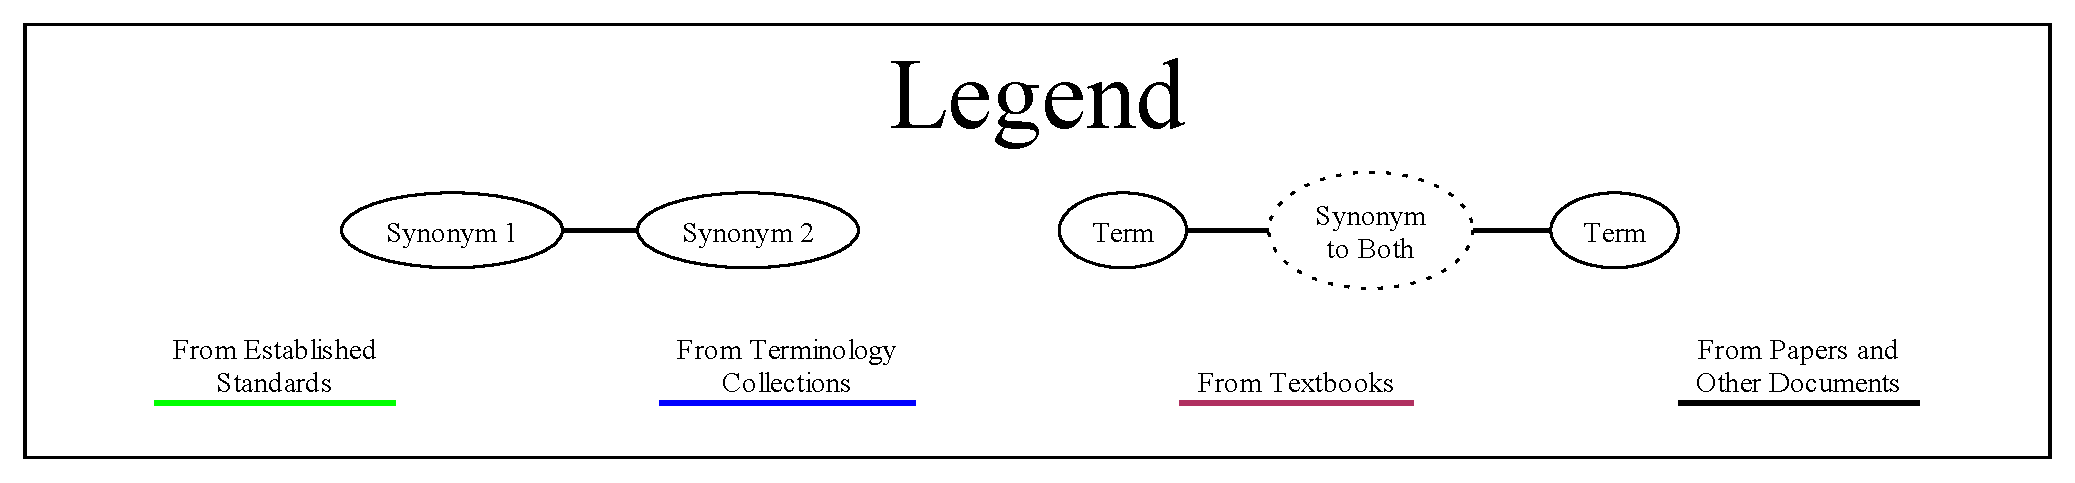
\includegraphics[width=\textwidth]{assets/graphs/manual/expSynLegend.pdf}
        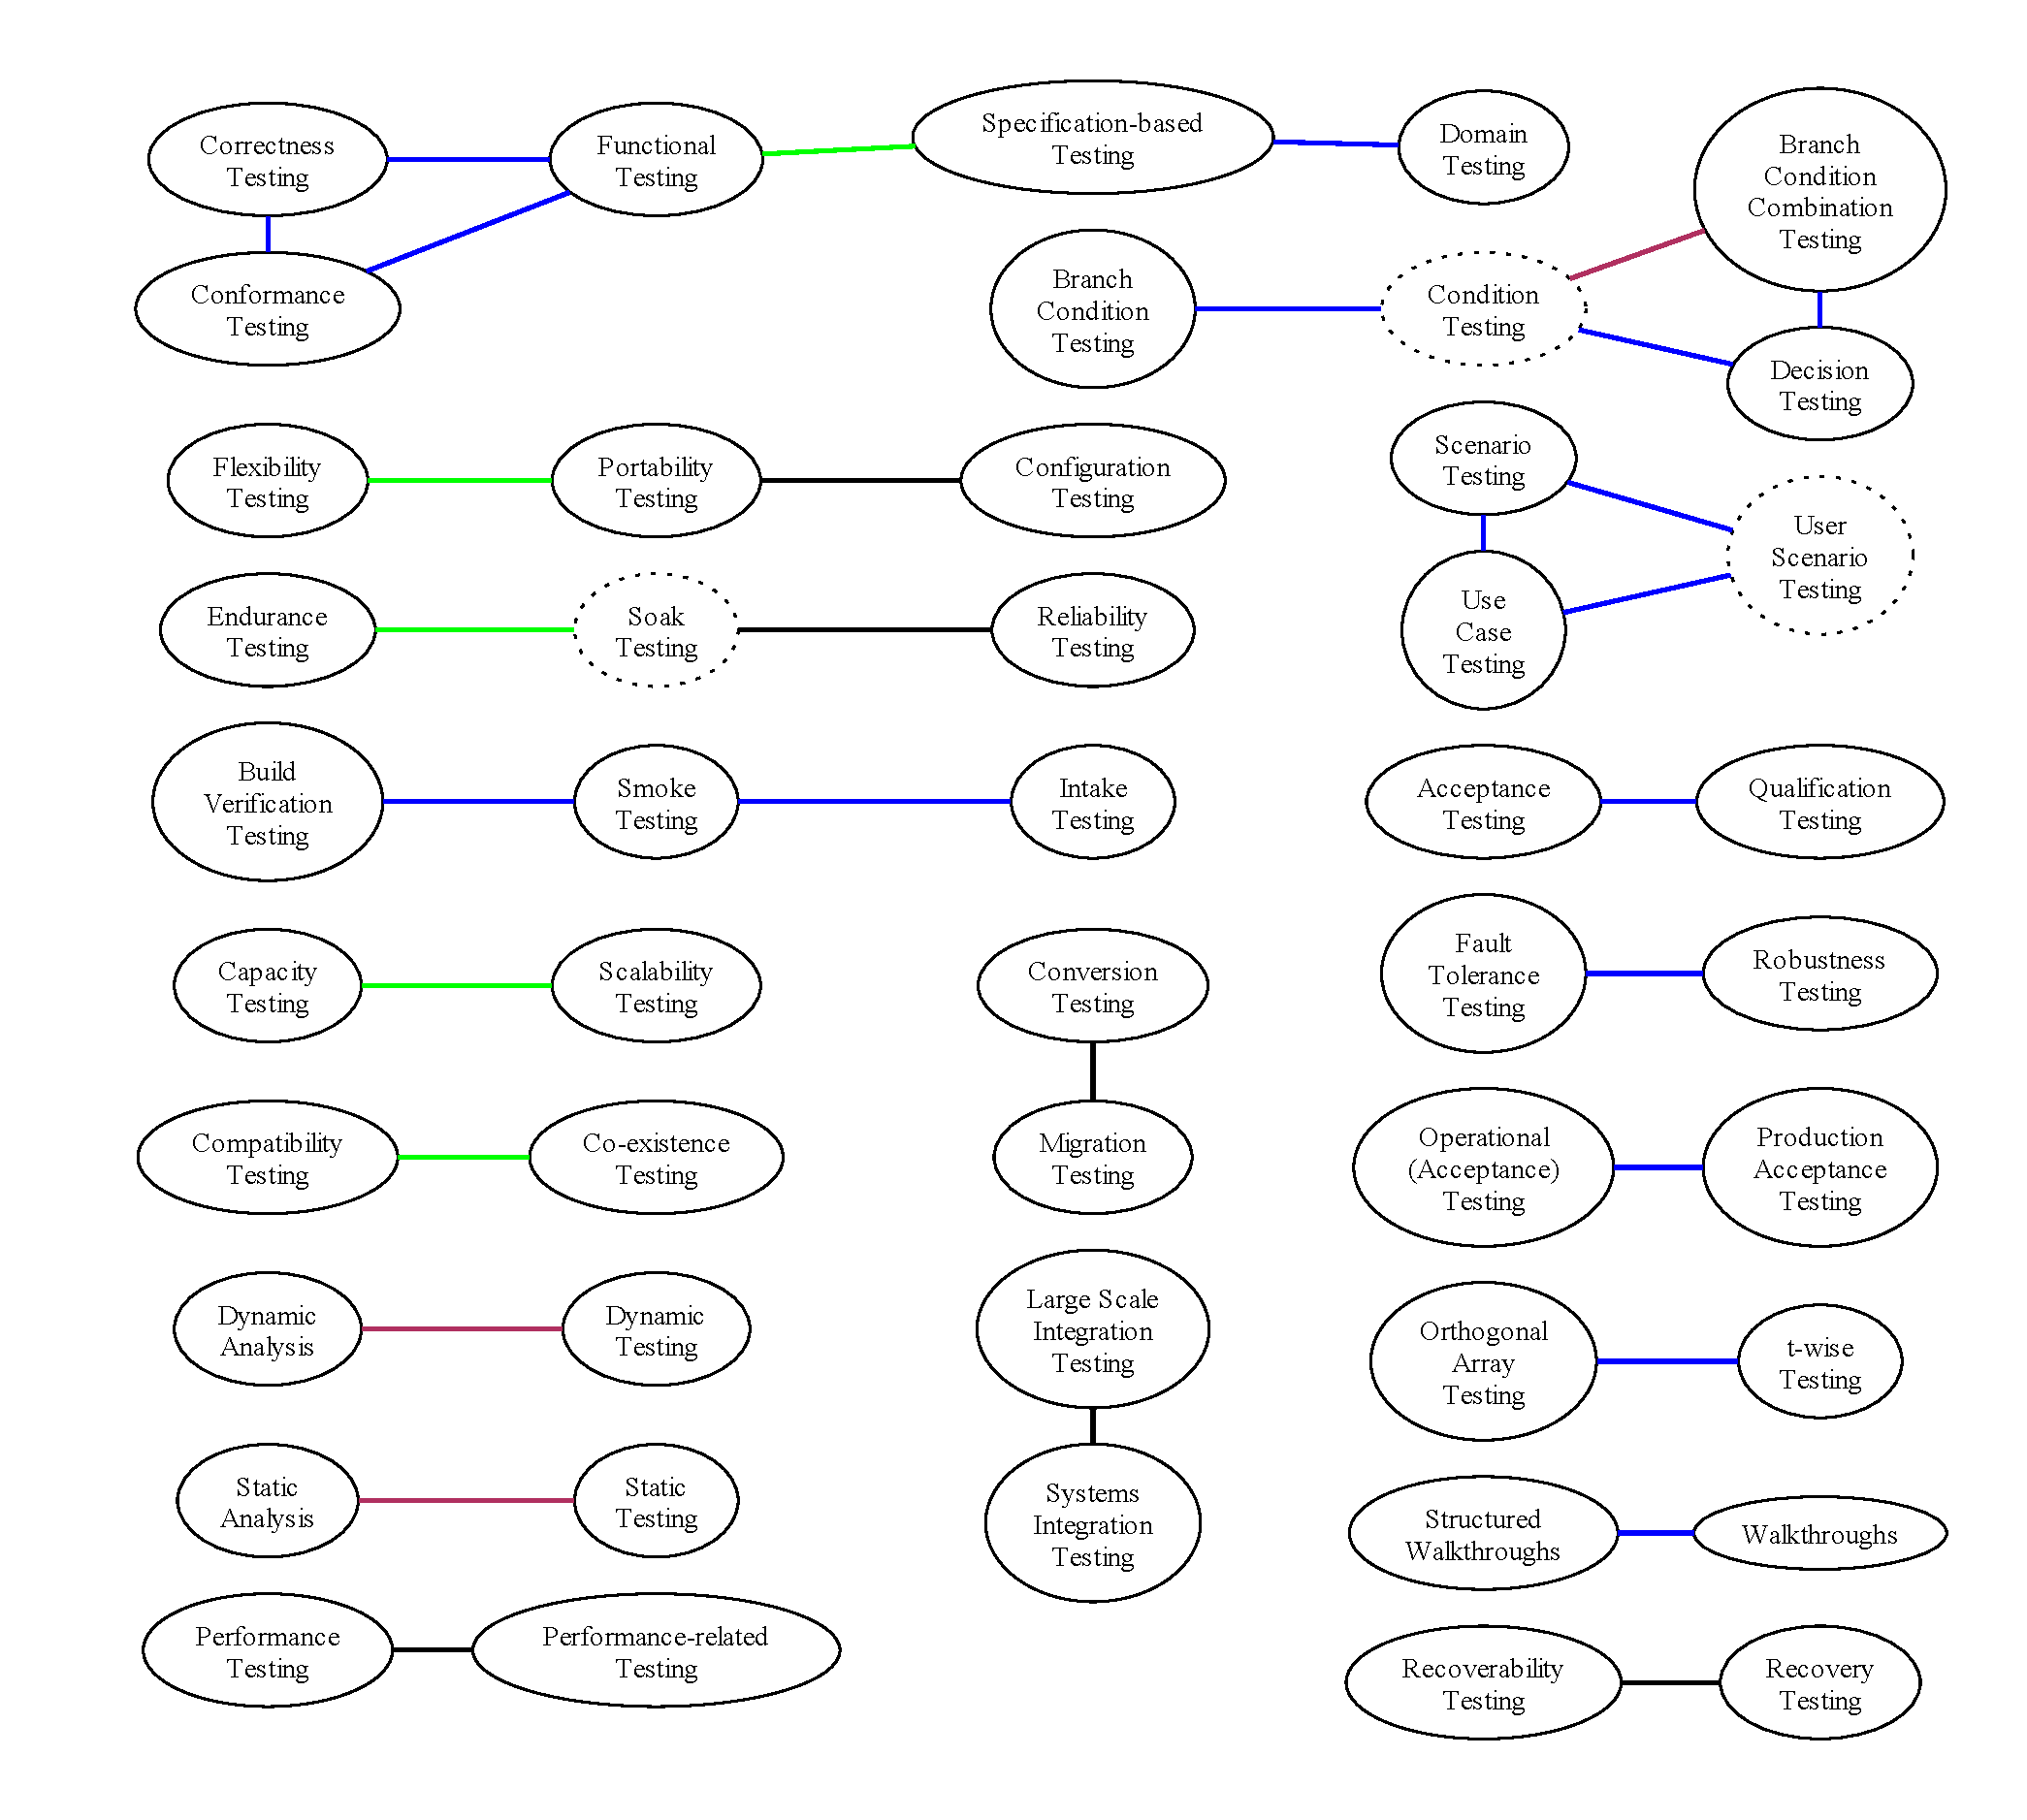
\includegraphics[width=\textwidth]{assets/graphs/manual/expSynGraph.pdf}
        % \vspace{-7mm}
        \caption{Visually meaningful \hyperref[syn-rels]{synonym} relations
            given explicitly by the literature.}\label{fig:expSynGraph}
    \end{figure}

    \begin{figure}[bt!]
        \centering
        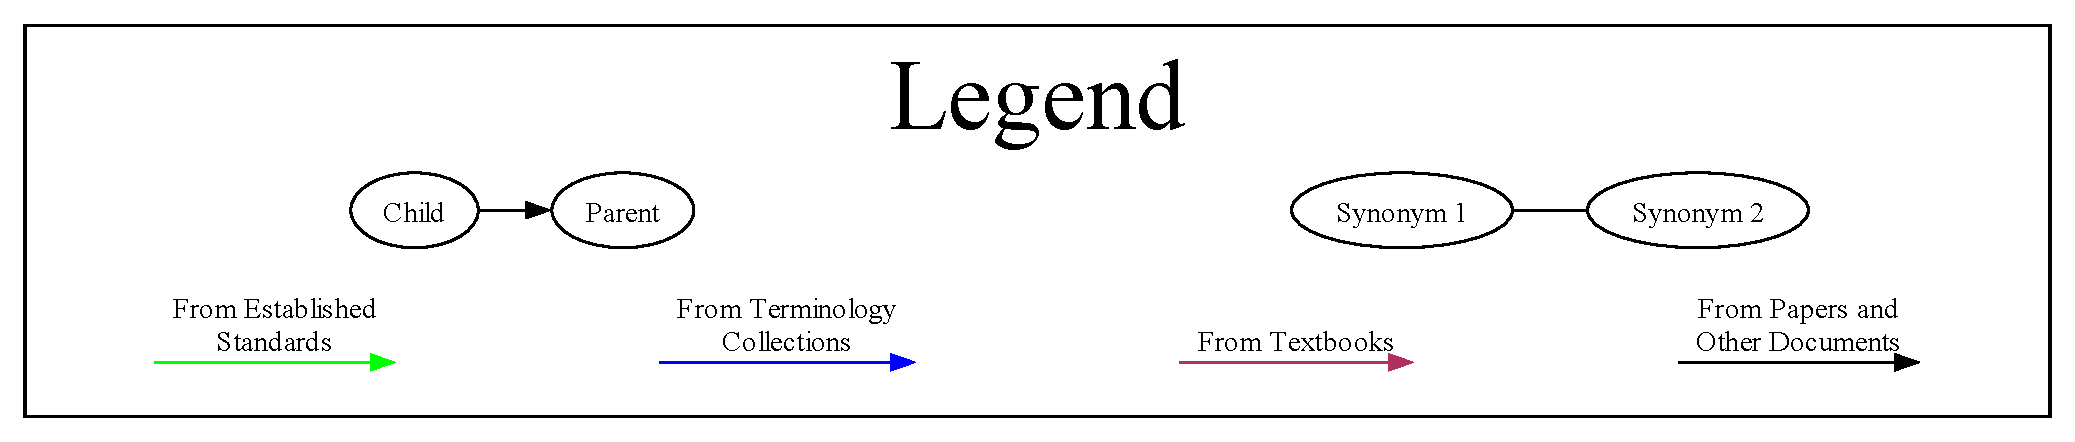
\includegraphics[width=0.48\linewidth]{assets/graphs/manual/expParSynLegend.pdf}
        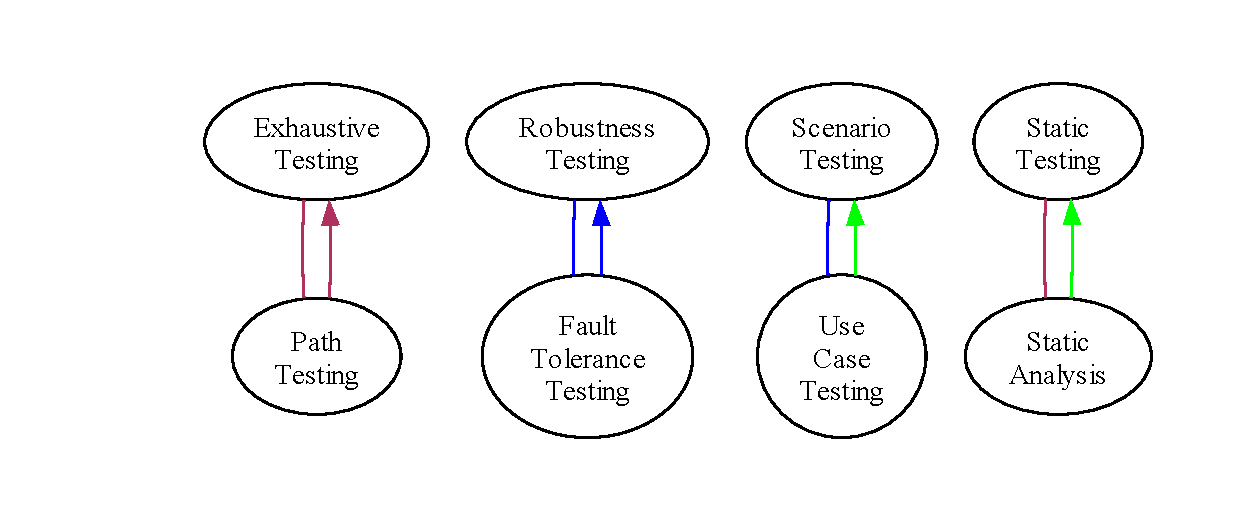
\includegraphics[width=0.5\linewidth]{assets/graphs/manual/expParSynGraph.pdf}
        % \vspace{-7mm}
        \caption{Pairs of test approaches with a \hyperref[par-chd-rels]{parent-child}
            \emph{and} \hyperref[syn-rels]{synonym} relation given explicitly by the
            literature.}\label{fig:expParSynGraph}
    \end{figure}
\else
\fi

\phantomsection{}\label{parSyns}
\parSynIntro{}\ifnotpaper. We visualize the pairs where both
relations are explicit in \Cref{fig:expParSynGraph} and list all
identified pairs in \Cref{tab:parSyns}, as well as pairs where we infer a
flaw in \Cref{infParSyns} for completeness\else\ and list the most
prominent in \Cref{tab:parSyns}\fi. Of
particular note is the relation between path testing and exhaustive testing.
While \citet[p.~421]{vanVliet2000} claims that path testing done completely
``is equivalent to exhaustively testing the program''\ifnotpaper\footnote{The
        contradictory definitions of path testing given in \flawref{path-test}
        add another layer of complexity to this claim.}\fi, this overlooks the
effects of input data \ifnotpaper
    (\citealp[pp.~129\==130]{IEEE2021c}; \citealp[p.~121]{Patton2006};
    \citealp[p.~467]{PetersAndPedrycz2000})
\else
    \cite[p.~467]{PetersAndPedrycz2000}, \cite[p.~121]{Patton2006},
    \cite[p.~129\==130]{IEEE2021c}
\fi and implementation issues \citetext{p.~476} % \citep[p.~476]{PetersAndPedrycz2000}
on the code's behaviour. Exhaustive testing
requires ``all combinations of input values \emph{and} preconditions \dots{}
[to be] tested'' \ifnotpaper (\citealp[p.~4, emphasis added]{IEEE2022};
    similar in \citealpISTQB{}; \citealp[p.~121]{Patton2006})\else
    \cite[p.~4]{IEEE2022} (similar in \citealpISTQB{},
    \cite[p.~121]{Patton2006})\fi.
% Flaw count (WRONG, SYNS): {vanVliet2000} | {IEEE2022} {IEEE2021c} ISTQB {PetersAndPedrycz2000} {Patton2006}

% % TODO: re-investigate this after going through the rest of ISO/IEC/IEEE 29119
% \ifnotpaper
%     \subsubsection{Definition Flaws}\label{defs}

%     \citet{IEEE2022, IEEE2021a, IEEE2021b, IEEE2021c}, from the
%     ISO/IEC/IEEE 29119 family of standards, mention the following 28 test
%     approaches without defining them. This means that out of the 119 test
%     approaches they mention, more than 20\% have no associated definition!

%     However, the previous version of this standard, \citeyearpar{IEEE2013},
%     generally explained two, provided references for two, and explicitly defined
%     one of these terms, for a total of five definitions that could (should) have
%     been included in \citeyearpar{IEEE2022}! These terms have been
%     \underline{underlined}\ifnotpaper%
%         , \emph{italicized}, and \textbf{bolded}, respectively%
%     \fi. Additionally, entries marked with an asterisk* were defined (at least
%     partially) in \citeyearpar{IEEE2017}, which would have been available when
%     creating this family of standards. These terms bring the total count of
%     terms that could (should) have been defined to eleven; almost 40\% of
%     these undefined test approaches could have been defined!

%     \begin{itemize}
%         \item \underline{Acceptance Testing*}
%         \item Alpha Testing*
%         \item Beta Testing*
%         \item BCP Testing
%         \item Capture-Replay Driven Testing
%         \item Configuration Testing*
%         \item Data-driven Testing
%         \item Error-based Testing
%         \item Factory Acceptance Testing
%         \item Fault Injection Testing
%         \item Functional Suitability Testing (also mentioned but not defined in
%               \citep{IEEE2017}; Functional Suitability*)
%         \item Inspections*
%         \item \underline{Integration Testing}*
%         \item Maintenance Testing
%         \item Model Verification
%         \item Operational Acceptance Testing
%         \item Orthogonal Array Testing
%         \item Peer Reviews
%         \item Production Verification Testing
%         \item Recovery Testing* (Failover/Recovery Testing, Back-up/Recovery
%               Testing, \formatPaper{\textbf}{Backup and Recovery Testing*},
%               Recovery*; see \Cref{recov-flaw})
%         \item Response-Time Testing
%         \item \formatPaper{\emph}{Reviews} (ISO/IEC 20246) (Code Reviews*)
%               (IEEE 1028, the IEEE ``Standard for Software Reviews and Audits'',
%               is cited in the bibliography!)
%         \item Scalability Testing (given as a synonym of ``capacity
%               testing''; see \Cref{scal-flaw})
%         \item Statistical Testing
%         \item System Integration Testing (System Integration*)
%         \item System Testing* (also mentioned but not defined in \citep{IEEE2013})
%         \item \formatPaper{\emph}{Unit Testing*}
%               (IEEE 1008, the IEEE ``Standard for Software Unit Testing'',
%               is cited in the bibliography!)
%         \item User Acceptance Testing
%     \end{itemize}
% \fi

\ifnotpaper
    \clearpage
    \subsection{Operational (Acceptance) Testing}\label{oat-flaw}
    \paragraph{\texttt{(CONTRA, LABELS)}}
    % Flaw count (CONTRA, LABELS): {IEEE2022} ISTQB | {SWEBOK2024} {ISO_IEC2018} {IEEE2017} {SWEBOK2014}
    There are two names that the literature gives to this test approach:
    \begin{itemize}
        \item \emph{\acf{operat}} (\citealp[p.~22]{IEEE2022};
              \citealpISTQB{}) and
        \item \emph{\acf{ot}} (\citealp{ISO_IEC2018};
              \citealp[p.~303]{IEEE2017}; \citealp[p.~6\=/9, in the context of
                  software engineering operations]{SWEBOK2024};
              \citealp[pp.~4\=/6, 4\=/9]{SWEBOK2014}).
    \end{itemize}

    \paragraph{\texttt{(CONTRA, SYNS)}}
    % Flaw count (CONTRA, SYNS): {Firesmith2015}
    % Assertion: {LambdaTest2024} {BocchinoAndHamilton1996}
    \refHelper \citet[p.~30]{Firesmith2015} lists the above terms separately,
    but they are considered synonyms elsewhere \citep{LambdaTest2024,
        BocchinoAndHamilton1996}\todo{find more academic sources}; since
    \citeauthor{Firesmith2015} does not define these terms, it is hard to
    evaluate \ifnotpaper his \else its \fi distinction.
\fi

\subsection{Recovery Testing}\label{recov-flaw}

``Recovery testing'' is ``testing \dots\ aimed at verifying
software restart capabilities after a system crash or other disaster''
\citep[p.~5\=/9]{SWEBOK2024} including ``recover[ing] the data directly affected
and re-establish[ing] the desired state of the system'' \ifnotpaper
    (\citealp{ISO_IEC2023a}; similar in \citealp[p.~7\=/10]{SWEBOK2024})
\else \cite{ISO_IEC2023a} (similar in \cite[p.~7\=/10]{SWEBOK2024}) \fi
so that the system ``can perform required functions'' \citep[p.~370]{IEEE2017}.
However, the literature also describes similar test approaches with vague or
non-existent distinctions between them. We describe these approaches and their
flaws here and present the relations between them in \Cref{fig:rec-graph-current}.

\NewDocumentCommand\subDRT{s}{given as a subtype of ``disaster/recovery
    testing'' which tests if ``operation of the test item can
    be transferred to a different operating site''
    \IfBooleanTF{#1}{\citetext{p.~37}}{\citeyearpar[p.~37]{IEEE2021c}},
    even though this is \emph{explicitly} excluded from its definition on the
    same page!}

%% again, maybe convert to \paragraph ?
\begin{itemize}
    \item \emph{Recoverability testing} evaluates ``how well a system or
          software can recover data during an interruption or failure''
          \ifnotpaper (\citealp[p.~7\=/10]{SWEBOK2024}; \else
              \cite[p.~7\=/10]{SWEBOK2024} (\fi similar in \citealp{ISO_IEC2023a})
          and ``re-establish the desired state of the system''
          \citeyearpar{ISO_IEC2023a}. \refHelper \citet[p.~47]{Kam2008}
          gives this as a synonym for ``recovery testing''.
    \item \emph{Disaster/recovery testing} evaluates if a system
          can ``return to normal operation after a hardware
          or software failure'' \citep[p.~140]{IEEE2017} or if ``operation of
          the test item can be transferred to a different operating site and
          \dots\ be transferred back again once the failure has been
          resolved'' \citeyearpar[p.~37]{IEEE2021c}.
          \begin{itemize}
              \item \texttt{(OVER, DEFS)}
                    % Flaw count (OVER, DEFS): {IEEE2017} | {IEEE2021c}
                    These two definitions seem to describe different aspects of
                    the system, where the first is intrinsic to the
                    hardware/software and the second might not be, making this
                    term nonatomic.
          \end{itemize}
    \item \emph{Backup and recovery testing} ``measures the
          degree to which system state can be restored from backup within
          specified parameters of time, cost, completeness, and accuracy in
          the event of failure'' \citep[p.~2]{IEEE2013}. This may be what is
          meant by ``recovery testing'' in the context of performance-related
          testing \citeyearpar[Fig.~2]{IEEE2022}.
    \item \emph{Backup/recovery testing} determines the ability of a system
          ``to restor[e] from back-up memory in the event of failure, without
          transfer[ing] to a different operating site or back-up system''
          \citep[p.~37]{IEEE2021c}.
          \begin{itemize}
              %   \item \texttt{(OVER, DEFS)}
              %         % Flaw count (OVER, DEFS): {IEEE2021c} | {IEEE2017}
              %         This definition corresponds to the first definition of
              %         ``disaster/recovery testing'' given by
              %         \citeyearpar[p.~140]{IEEE2017}.
              \item \texttt{(CONTRA, PARS)}
                    % Flaw count (CONTRA, PARS): {IEEE2021c} | {IEEE2021c}
                    This \subDRT{}
              \item \texttt{(OVER, LABELS)}
                    % Flaw count (OVER, LABELS): {IEEE2021c} | {IEEE2013}
                    Its name is also quite similar to ``backup and
                    recovery testing'', adding further confusion.
          \end{itemize}
    \item \emph{Failover/recovery testing} determines the
          ability ``to mov[e] to a back-up system in the event of failure,
          without transfer[ing] to a different operating site''
          \citep[p.~37]{IEEE2021c}.
          \begin{itemize}
              \item \texttt{(CONTRA, PARS)}
                    % Flaw count (CONTRA, PARS): {IEEE2021c} | {IEEE2021c}
                    This is also \subDRT*{}
              \item \texttt{(AMBI, PARS)}
                    % Flaw count (AMBI, PARS): {IEEE2021c}
                    % Assertion: {SWEBOK2024} ISTQB
                    While not explicitly related to recovery, \emph{failover
                        testing} ``validates the SUT's ability to manage heavy
                    loads or unexpected failure to continue typical operations''
                    \citep[p.~5\=/9]{SWEBOK2024} by entering a ``backup
                    operational mode in which [these responsibilities] \dots\
                    are assumed by a secondary system'' \citepISTQB{}. Its name
                    implies that it is a child of ``failover/recovery testing''
                    but its definition makes it more broad (as it includes handling
                    ``heavy loads'' where failover/recovery testing does not)
                    which may reverse the direction of this relation.
              \item \texttt{(AMBI, SYNS)}
                    % Flaw count (AMBI, SYNS): {IEEE2021c} | implied by {Firesmith2015}
                    \refHelper \citet[p.~56]{Firesmith2015} uses the term
                    ``failover and recovery testing'' which may be a synonym of
                    ``failover/recovery testing''.
          \end{itemize}
    \item \emph{Restart \& recovery (testing)} is listed as a test approach by
          \citet[Fig.~5]{Gerrard2000a} but is not defined \texttt{(MISS, DEFS)}
          % Flaw count (MISS, DEFS): {Gerrard2000a}
          and may simply be a synonym to ``recovery testing'' \texttt{(AMBI, SYNS)}.
          % Flaw count (AMBI, SYNS): {Gerrard2000a}
\end{itemize}

\subsection{Scalability Testing}\label{scal-flaw}

\paragraph{\texttt{(CONTRA, SYNS)}}

% Flaw count (CONTRA, SYNS): {IEEE2021c} | {Firesmith2015} {Bas2024}
\citeauthor{IEEE2021c} \citeyearpar[p.~39]{IEEE2021c} give
``scalability testing'' as a synonym of ``capacity testing''
while other sources differentiate between the two \ifnotpaper
    (\citealp[p.~53]{Firesmith2015}; \citealp[pp.~22\==23]{Bas2024})%
\else \cite[p.~53]{Firesmith2015}, \cite[pp.~22\==23]{Bas2024}\fi.

\paragraph{\texttt{(CONTRA, DEFS)}}

% Flaw count (CONTRA, DEFS): {IEEE2021c} | implied by {ISO_IEC2023a}
\citeauthor{IEEE2021c} \citeyearpar[p.~39]{IEEE2021c} also include the external
modification of the system as part of ``scalability'' but
\citet{ISO_IEC2023a} \multiAuthHelper{describe} it as testing the ``capability
of a product to handle growing or shrinking workloads or to adapt its capacity
to handle variability'', implying that this is done by the system itself.

\paragraph{\texttt{(WRONG, LABELS)}}

% Flaw count (WRONG, LABELS): {SWEBOK2024}
\citeauthor{SWEBOK2024} \citeyearpar[p.~5\=/9]{SWEBOK2024} says ``scalability
testing evaluates the capability to use and learn the system and the user
documentation'' and ``focuses on the system's effectiveness in supporting user
tasks and the ability to recover from user errors''. \swebokScalDef{}.

% \subsection{Performance Testing}
% \label{perf-test-ambiguity}

% Similarly, ``performance'' and ``performance efficiency'' are both given as
% software qualities by \ifnotpaper\citeauthor{IEEE2017}\else
%       \cite[p.~319]{IEEE2017}\fi, with the latter defined as the ``performance
% relative to the amount of resources used under stated conditions''
% \ifnotpaper\citeyearpar[p.~319]{IEEE2017} \fi or the ``capability of a product
% to perform its functions within specified time and throughput parameters and be
% efficient in the use of resources under specified conditions'' \citep{ISO_IEC2023a}.
% Initially, there didn't seem to be any meaningful distinction between the two,
% although the term ``performance testing'' is defined
% \ifnotpaper\citeyearpar[p.~320]{IEEE2017}\else\citetext{p.~320}\fi\
% and used by \ifnotpaper\citeauthor{IEEE2017}\else\cite{IEEE2017}\fi\ and the term
% ``performance efficiency testing'' is \emph{also} used by
% \ifnotpaper\citeauthor{IEEE2017}\else\cite{IEEE2017}\fi\ (but not defined
% explicitly). \ifnotpaper Further discussion\thesisissueref{43} brought us to
%       the conclusion \else It can then be concluded \fi that ``performance
% efficiency testing'' is a subset of ``performance testing'', and the
% difference of ``relative to the amount of resources used'' or ``be efficient in
% the use of resources'' between the two is meaningful.

\subsection{Compatibility Testing}\label{compat-flaw}

\paragraph{\texttt{(OVER, DEFS)}}
% Flaw count (OVER, DEFS): {IEEE2022} | {IEEE2017} ISTQB {ISO_IEC2023a}
``Compatibility testing'' is defined as ``testing that measures the
degree to which a test item can function satisfactorily alongside
other independent products in a shared environment (co-existence),
and where necessary, exchanges information with other systems or
components (interoperability)'' \citep[p.~3]{IEEE2022}. This
definition is nonatomic as it combines the ideas of ``co-existence''
and ``interoperability''.

\paragraph{\texttt{(WRONG, SYNS)}}
% Flaw count (WRONG, SYNS): implied by {IEEE2021c} | {IEEE2022}
The ``interoperability'' element of ``compatibility testing'' is explicitly
excluded by \citet[p.~37]{IEEE2021c}, (incorrectly) implying that ``compatibility
testing'' and ``co-existence testing'' are synonyms.

\paragraph{\texttt{(AMBI, SYNS)}}
% Flaw count (AMBI, SYNS): {Kam2008} | {IEEE2022}
Furthermore, the definition of ``compatibility testing'' in
\citet[p.~43]{Kam2008} unhelpfully says ``see \emph{interoperability testing}'',
adding another layer of confusion to the direction of their relationship.

\paragraph{\texttt{(WRONG, LABELS)}}
% Flaw count (WRONG, LABELS): {IEEE2022}
% Assertion: {ISO_IEC2023a} {IEEE2022} {IEEE2021c} {IEEE2017} ISTQB
\refHelper \citet[pp.~22, 43]{IEEE2022} \multiAuthHelper{say}
``interoperability testing helps confirm that applications can work on multiple
operating systems and devices'', but this seems to instead describe
``portability testing'', which evaluates the ``capability of a product to be
adapted to changes in its requirements, contexts of use, or system environment''
\ifnotpaper
    (\citealp{ISO_IEC2023a}; similar in \citealp[p.~7]{IEEE2022};
    \citeyear[pp.~184, 329]{IEEE2017}; \citealpISTQB{})\else
    \cite{ISO_IEC2023a} (similar in \citeyear[pp.~184, 329]{IEEE2017},
    \citealp[p.~7]{IEEE2022}, \cite{ISTQB})\fi, such as being ``transferred
from one hardware \dots{} environment to another'' \citep[p.~39]{IEEE2021c}.
